\section{Materials and Methods}

\subsection{Data Collection}

\textbf{CAUEEG-Dementia.} CAUEEG \citep{kim2023caueeg} contains clinical 19-channel scalp EEG (international
10--20 system) recorded at 200\,Hz at Chung-Ang University Hospital, Korea, with event annotations for eyes
open/closed, photic stimulation, hyperventilation, artifacts and recording pauses. The dementia task has
1,187 recordings (459 Normal, 417 MCI, 311 Dementia) in an official split of 950 training, 119 validation and
118 test recordings. The official \textit{no-overlap} test subset (90 recordings) excludes patients who also
have recordings in the training split. Using the dataset's symptom codes, the Normal class divides into
community-recruited volunteers, patients with subjective memory impairment (SMI) whose testing was normal, and
13 recordings with neither code (Table~\ref{tab:groups}).

\begin{table}[H]
\centering
\caption{CAUEEG-Dementia subgroups (all 1,187 recordings)}
\label{tab:groups}
\small
\begin{tabular}{lrcccccc}
\toprule
Group & $n$ & Age (years) & Photic (\%) & EO (\%) & Length (min) & EC (min) & Photic (min)\\
\midrule
Normal: community & 260 & $61.7\pm8.3$ & 12 & 63 & 10.2 & 5.7 & 0.1\\
Normal: SMI & 186 & $69.6\pm9.3$ & 90 & 84 & 13.8 & 5.6 & 0.7\\
Normal: other & 13 & $68.4\pm7.2$ & 69 & 85 & 13.2 & 5.5 & 0.6\\
MCI & 417 & $73.8\pm7.8$ & 92 & 87 & 13.8 & 5.8 & 0.8\\
Dementia & 311 & $76.6\pm8.1$ & 92 & 80 & 14.0 & 6.6 & 0.8\\
\bottomrule
\end{tabular}\\[2pt]
\parbox{\textwidth}{\scriptsize Photic / EO: share of recordings with usable photic-stimulation / eyes-open data.
EC: eyes closed. Durations are clean minutes after artifact masking.}
\end{table}

\textbf{External cohorts.} For testing without retraining we use two public MCI datasets. \textbf{Isfahan}
\citep{kashefpoor2016automatic,kashefpoor2019supervised} has two releases of 19-channel, 256\,Hz eyes-closed
resting EEG (2016: 16 normal / 11 MCI; 2019: 16 normal / 18 MCI). \textbf{GENEEG} \citep{geneeg2025} has
general-practice recordings (35 control / 28 MCI) at 250\,Hz during an eyes-closed P300 protocol, with the T5
and T6 channels unavailable (interpolated). Neither provides state annotations or per-subject ages, so all
segments are treated as one state and a fixed age is imputed, which removes age as a source of information.

\subsection{Preprocessing}
Signals are band-pass filtered (0.5--45\,Hz, fourth-order zero-phase Butterworth), clipped at $\pm3000\,\mu$V
and resampled to 100\,Hz. The first 10\,s are discarded for electrode settling. External recordings are
re-referenced to the common average, as in CAUEEG.

\textbf{Event-clock correction.} Each CAUEEG event is a sample index at 200\,Hz with a text label. These indices
count wall-clock time \emph{including} paused periods, whereas the EDF signal contains only the recorded
portions joined end-to-end. Event $i$ therefore maps to signal position
\begin{equation}
\hat{t}_i = t_i - \sum_{p:\, r_p \le t_i} (r_p - s_p),
\end{equation}
where $s_p$ and $r_p$ are the \textit{Paused} and \textit{Recording resumed} indices of pause $p$. Every
recording ends with a \textit{Paused} event, which should coincide with the end of the signal and so checks
the alignment. Of the 1,187 recordings, 293 contain a pause. In these, the raw final event lies a median of
33\,s (maximum 678\,s) from the signal end; after correction the median is 3\,s, and 1,184 of 1,186 recordings
align within 6\,s (Figure~\ref{fig:align}).

\begin{figure}[H]
\centering
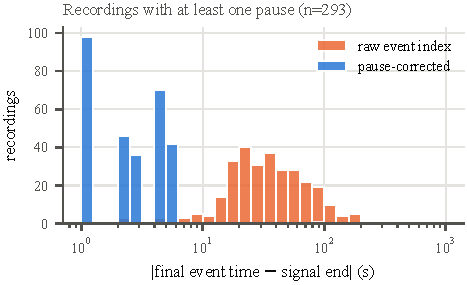
\includegraphics[width=0.7\textwidth]{figures/alignment.pdf}
\caption{Offset between the final \textit{Paused} event and the end of the signal for recordings with
pauses, before (orange) and after (blue) the correction.}
\label{fig:align}
\end{figure}

\textbf{State timeline and clean mask.} From the corrected events we label every second as eyes-closed,
eyes-open, photic, hyperventilation or unknown. A clean mask removes 1\,s before and 3\,s after every state
change, 3\,s around pause joins, 2\,s before to 3\,s after point artifacts (movement, coughing, swallowing,
talking) and 30\,s after drowsiness or sleep annotations. Hyperventilation, which slows the EEG of healthy
subjects, is excluded from both segments and biomarkers.

\subsection{Age-Normative Clinical Biomarkers}
For each recording we compute 48 biomarkers from Welch spectra of 4\,s windows (2\,s step):
\begin{itemize}[leftmargin=*,itemsep=0pt,topsep=2pt]
\item \textit{Eyes-closed (39):} log relative $\delta$, $\theta$, $\alpha$ and $\beta$ power in five regions;
      theta/alpha, delta/alpha and slow/fast ratios; fronto-posterior alpha ratio; alpha and beta hemispheric
      asymmetry; posterior alpha centre of gravity and peak frequency; spectral entropy; median frequency;
      total power; Hjorth mobility and complexity; inter-hemispheric and fronto-posterior coherence.
\item \textit{Eyes-open (5):} global relative band powers and posterior alpha centre of gravity.
\item \textit{Reactivity and driving (2):} posterior alpha reactivity, $\log(P_\alpha^{EC}/P_\alpha^{EO})$, and
      occipital photic-driving signal-to-noise ratio at the flash frequency.
\item \textit{Availability (2):} indicators for the presence of eyes-open and photic data.
\end{itemize}
Because EEG slows with healthy ageing, a raw biomarker mixes age with impairment. For every biomarker $x_j$ we
fit a linear age model on the \emph{training Normal recordings only} and replace $x_j$ with its robust
deviation
\begin{equation}
z_j = \frac{x_j - f_j(\text{age})}{1.4826\,\mathrm{MAD}_j},
\end{equation}
where $\mathrm{MAD}_j$ is the median absolute deviation of the normal residuals; values are clipped to
$\pm6$. In cross-validation the normative model is refitted within each fold.

\subsection{Evaluation Protocol}
All metrics are per recording and all splits are patient-disjoint. We report two complementary protocols.
(i) \textbf{Official split}, the benchmark protocol of \citet{kim2023caueeg}: models are trained on the 950
training recordings and scored on the 118 test recordings and the 90-recording no-overlap subset.
(ii) \textbf{Repeated five-fold cross-validation} over the pooled 1,069 training and validation recordings,
with the normative model and age scaling refitted in each fold, giving one out-of-fold prediction per
recording; the main models are run with several fold assignments. Metrics are accuracy, balanced accuracy,
macro F1, macro one-vs-rest area under the ROC curve (AUC), per-class recall and pairwise AUCs, with 95\%
bootstrap confidence intervals (1,000 resamples); model differences use a paired bootstrap on the same
recordings.
